\section{Autocrop mechanism for inference}
\label{sec:autocrop}

This section gives a detailed description of the so-called autocrop.
This cropping mechanism is responsible for cutting out the desired input for the model in inference.
First, the autocrop from \cite{tepNet2024} is described in detail.
Furthermore, an improved version of this cropping mechanism is explained.

\subsection{Autocrop for inference with TEP's cropping mechanism}

In \cite{tepNet2024}, only cropped images are used for training models to only consider the most relevant \ac{ROI} in images.
For training and validating the model on the dataset, the \ac{GT} allows the computation of crop coordinates (left, top, right).
However, \ac{GT} data is unavailable in practical applications like video inference.
As a result, the crop coordinates must be predefined by a user or computed on the fly.

In a real-world application, the \ac{ROI} in the images changes, even when the camera is mounted in a fixed position.
Because of these perspective shifts, when the train drives right or left turns, it quickly can become unsustainable to have predetermined crop coordinates.
\autoref{fig:perspective_shifts} visualizes these perspective shifts.
The tighter the curve, the worse the shift.
The approach of \cite{tepNet2024} to solve this particular problem is the so-called "Autocrop".
This developed technique starts with the whole image, so the initial crop coordinates are the image borders.
After the initialization, the three coordinates (left, top, right) are updated according to the prediction of every new frame.
In more detail, new coordinates are calculated with a \ac{RA} of the smallest rectangle around the prediction plus the predefined margins from the training.
Furthermore, the global averages of crop coordinates are taken into consideration.
This allows the crop coordinates to converge to these global averages and prevent collapse scenarios in which the crop becomes too small.


\begin{figure}[H]
    \centering
    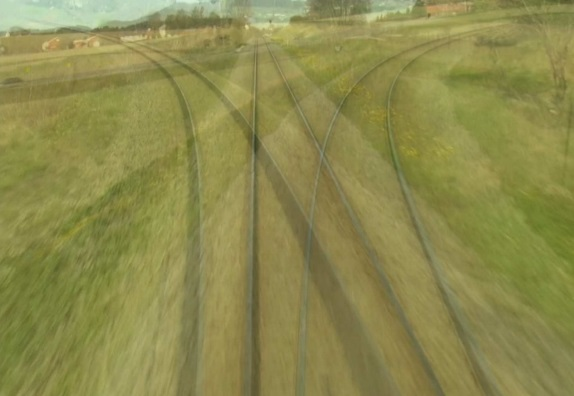
\includegraphics[width=0.7\linewidth]{PICs/Baselinepaper/perspective_shifts.jpg}
    \caption{Example of perspective shifts with three different scenarios: left curve, right curve, and straight rail \cite{tepNet2024}.}
    \label{fig:perspective_shifts}
\end{figure}

\subsection{Improved Autocrop for inference}
\label{sec:imporvedAutocrop}

\cite{tepNet2024} incorporates a \ac{RA} (\autoref{func:runningAverage}) with rule-based policies to prevent collapse to the inside and consider image borders when adding a margin. After that, the newly calculated and checked average is weighted and added to form the new crop coordinates, like in \autoref{func:weightingAverage}. In these formulas, $AVG$ is the average, $x$ is the crop coordinates, and $pred$ are the values obtained from the prediction. In \autoref{func:weightingAverage}, the same annotations are used with $c$ being the coefficient, which is 0.1. All notations but $c$ include all three crop coordinates: left, top right.

\begin{align}
    AVG_t = \frac{AVG_{t-1} \cdot (t-1) + pred_t}{t}
    \label{func:runningAverage}
\end{align}

\begin{align}
    x_{t} = x_{t-1} * (1 - c) + AVG_{t} * c
    \label{func:weightingAverage}
\end{align}

\noindent However, observations in the inference of videos demonstrate that the introduced autocrop mechanism is not optimal. The behavior shows that the \ac{RA} reacts slowly when expanding or shrinking the input crop. This is especially problematic when the crop should quickly expand in one direction because of the given situation. Additionally, the borders of the crop converge to an overall average, presenting the same issues as when simply predefining a crop. Those behaviors can push the prediction outside the rails, especially in the case of a perspective shift. This happens when the train takes a curve, and the rails move to the left or right in the image. If the autocrop does not react quickly enough in this situation, the rails are subsequently positioned outside the crop area. An additional issue presents the lack of a recovery option when the image crop is completely incorrect.

\begin{align}
    x_t =  x_{t-1} * (1 - c) + pred_t * c
    \label{func:EMA}
\end{align}

\vspace{0.7cm}

\noindent Therefore, a new algorithm is implemented for this work to present a more robust solution.
The desired behavior should be more responsive to the outside to react to rapid changes in perspective.
Simultaneously, the crop should converge gradually to the inside to prevent any fast movements of crop coordinates, possibly leading to collapse events.

An \ac{EMA} is utilized to realize such an algorithm, shown in \autoref{func:EMA}, in which only the old crop coordinates and the values from the prediction are weighted and added.
$c$ is the coefficient set to 0.01, presenting slow movements to the inside.
Additionally, with the same collapse prevention technique as before, the crop cannot be smaller than the smallest rectangle of the prediction (yellow box in \autoref{fig:tepNet_dataaugmentation}).
However, directly calculating the crop coordinates without any averages in between, like \autoref{func:runningAverage}, leads to a different behavior.
The collapse prevention rule now overwrites the coordinates when the prediction expands, rapidly widening the crop.

Furthermore, the crop is bound to stay within image borders.
Further adaptations to enhance robustness are made by increasing the margins, which are added to the prediction rectangle (yellow box in \autoref{fig:tepNet_dataaugmentation}) to give the model more leeway.

A reset rule is also implemented in which the crop coordinates are overwritten with predefined values.
The behavior is observed that when models become uncertain, the horizon line converges to the bottom of the image.
This behavior is exploited, and the crop resets when the predicted horizon line is below 40\% of the crop height.
Experiments show that the following reset values are the most advantageous: left = 1/3 of image width, top = 1/2 of image height, right = 2/3 of image width.

\clearpage

\section{Data augmentation}
\label{sec:dataaugmentation}

This section gives a thorough explanation of the data augmentation of \cite{tepNet2024}.
Additionally, the adapted data augmentation for training temporal models is described in detail.

\subsection{Data augmentation for Training single-frame-based models}

\cite{tepNet2024} utilizes three data augmentation techniques in the training process.
The first two are commonly used in \ac{CV} tasks, including random horizontal flips and traditional image adjustments like brightness, contrast, saturation, and hue variations.
For this, the standard ColorJitter \cite{pytorch_colorJitter_docu} method from PyTorch is used.
The third augmentation is the cropping mechanism, which reduces the image to the most relevant part.
Randomness is also introduced to enhance generalization.

\autoref{fig:tepNet_dataaugmentation} visualizes the cropping algorithm steps schematically.
The \ac{GT} is in the form of polylines and is represented by the two green lines.
Then, the yellow rectangle is computed, being the smallest possible rectangle around the \ac{GT}.
In the next step, the start pixels of the rails \ac{GT} are centered by expanding the yellow borders in one direction, resulting in the orange box.
In the dataset, all start pixels of rails are in the lowest row of an image.
After that, margins are added, shown by the red rectangle.
These margins are predefined with hyperparameters.
After calculating the borders of the outermost box, variability is added to enhance generalization and prevent biases.
The left, right, and top borders are moved by a distance calculated with a predefined normal distribution.
This introduced variability follows the policy, ensuring that the rails' starting pixels at the bottom stay in the cropped image.
\autoref{fig:tepNet_dataaugmentation} illustrates four augmented variations of the top image in the bottom row.

\begin{figure}[H]
    \centering
    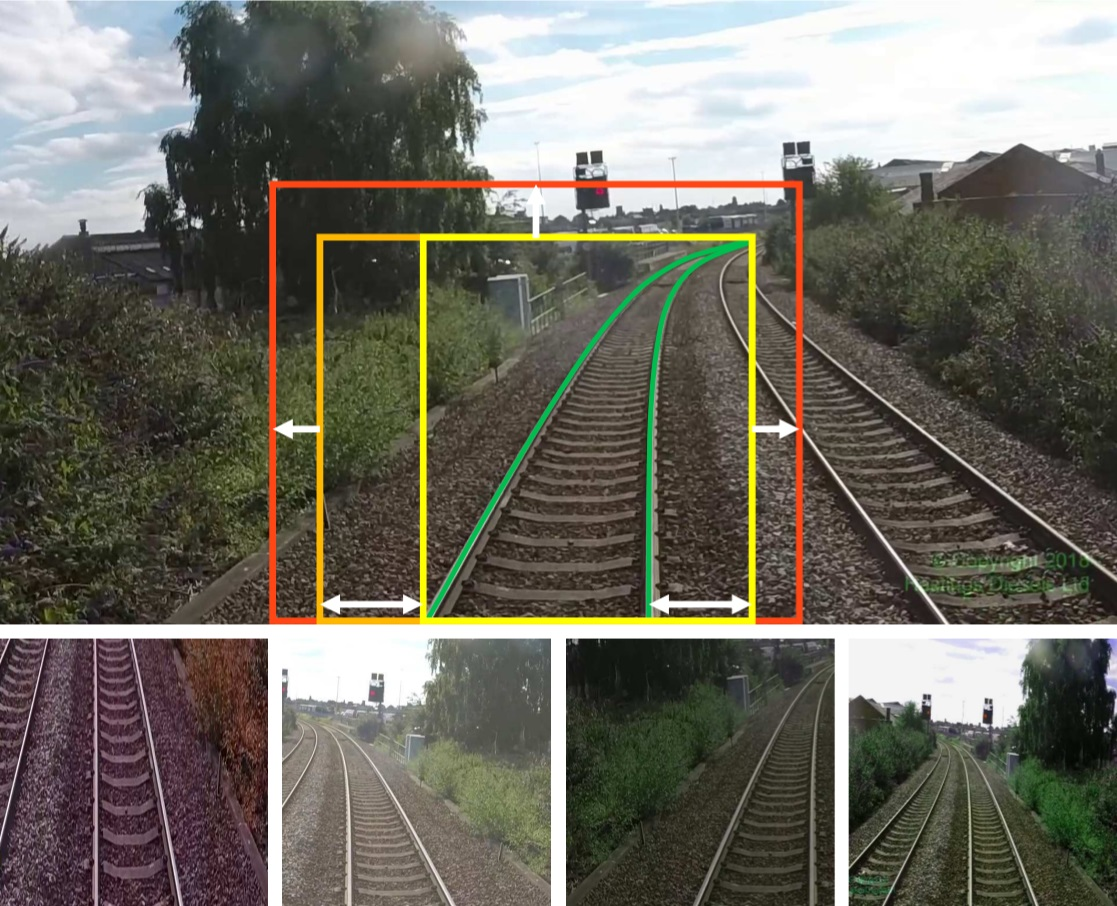
\includegraphics[width=0.6\linewidth]{PICs/Baselinepaper/data_augmenation.jpg}
    \caption{Data augmentation of \ac{TEP}-Net \cite{tepNet2024}, including the image horizontal flips, the color variations, and the cropping mechanism.}
    \label{fig:tepNet_dataaugmentation}
\end{figure}

\subsection{Data augmentation for Training temporal models}
\label{sec:dataAugmentationTemporal}

For training temporal models, the same three data augmentation strategies as the ones from training single-frame-based models are utilized for enhanced generalization.
These again include horizontal flips, color variations, and a similar cropping mechanism.
However, when training a model with sequences of images, the same augmentation must be used on all images of this sequence.
For the first two augmentation techniques, random values are obtained and saved in variables.
Then, these random factors are applied to each image in the sequence.
For the horizontal flip, a threshold at $0.5$ and a random value between $0$ and $1$ define whether a sequence is flipped.
To achieve the same effect as the ColorJitter \cite{pytorch_colorJitter_docu} function from the single-frame training, four uniform distributions output random values for brightness, contrast, saturation, and hue.
These are then the parameters for the functions: \texttt{adjust\_brightness} \cite{pytorch_adjust_brightness_docu}, \texttt{adjust\_contrast} \cite{pytorch_adjust_contrast_docu}, \texttt{adjust\_saturation} \cite{pytorch_adjust_saturation_docu}, and \texttt{adjust\_hue} \cite{pytorch_adjust_hue_docu}.

The cropping mechanism needs more consideration.
First, the same method as the one from single-frame training is applied to the first image of a sequence to obtain the red borders shown in \autoref{fig:tepNet_dataaugmentation}.
To still guarantee randomness and minimize the risk of unwanted biases, the location of the left, right, and top borders are moved according to a normal distribution.
The distances between the red and random borders are calculated to ensure consistency along a sequence.
From this point on, the red borders are calculated in every image as before, and these distances are used to incorporate random factors instead of new random values for every image.
The whole algorithm still follows a policy that the starting pixels of the rails stay in the image crop.
\autoref{fig:temporalDataAugmentation} visualizes an example sequence with raw images in the top row and augmented crops in the bottom row.
The first, middle, and last images of a sequence with 10 images are shown.
The train's progress is most clearly visible through the pole of the overhead line. 

\begin{figure}[H]
    \centering
    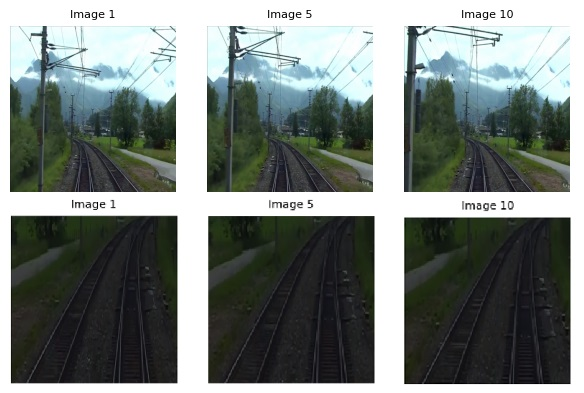
\includegraphics[width=0.59\linewidth]{PICs//dataAugmentation/temporal_data_augmentation.jpg}
    \caption{Data augmentation for temporal data processing, including the 1\textsuperscript{st}, 5\textsuperscript{th} and 10\textsuperscript{th} image of a sequence. The first row shows resized raw images. The second row depicts augmented images with the same three augmentation techniques for the whole sequence.}
    \label{fig:temporalDataAugmentation}
\end{figure}
